
\begin{figure*}[t]
    \centering
     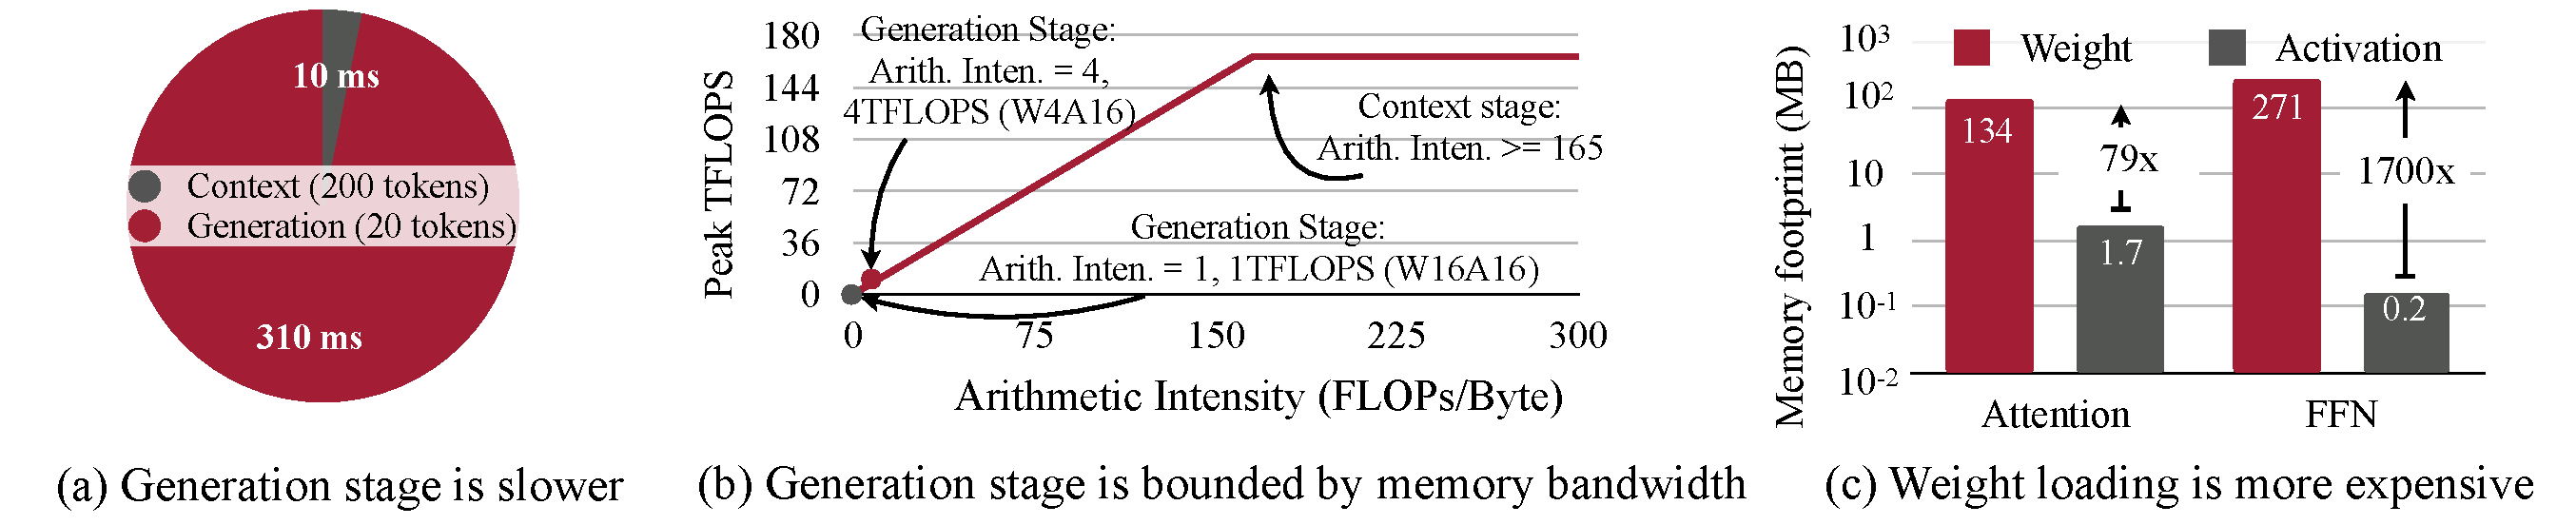
\includegraphics[width=\textwidth]{figures/memory_bound_analysis.pdf}
    \caption{Bottleneck analysis for Llama-2-7B on NVIDIA RTX 4090. \textbf{Left}: In on-device LLM applications, generation stage is much slower than the context stage. \textbf{Middle}: The generation stage is memory bound and has low arithmetic intensity. W4A16 quantization can effectively improve the arithmetic intensity by 4$\times$. \textbf{Right}: The amount of weight access is orders of magnitude larger than the amount of activation access. Thus, weight-only quantization is more effective for on-device LLMs.} 
    \label{fig:memory_bound_analysis}
\end{figure*}
